\section{Methods}

\begin{frame}
	\frametitle{Methods}
	\framesubtitle{Data representation}
	\begin{itemize}
		\item Treat every image as a 3D-tensor (RGB)
			\begin{itemize}
				\item Repeat the value of grayscale images three times
				\item Colorized are handled as the original tensors
			\end{itemize}
		\item Original data has 14 labels, we used 15
			\begin{itemize}
				\item Extra one for the unclassified images
				\item One-hot encoded labels
			\end{itemize}
	\end{itemize}
\end{frame}


\begin{frame}
	\frametitle{Methods}
	\framesubtitle{Data processing}
	\begin{itemize}
		\item Read images in batches of size 2000
		\begin{itemize}
			\item Helps to avoid filling the RAM
		\end{itemize}
		\item Normalize the pixel values between $[0.0, 1.0]$
		\item For every batch augmenting the data
		\begin{itemize}
			\item Provided by Keras
			\item Centerify, shear, zoom, rotate and flip
			\item To get more variation and samples from classes with few labels
		\end{itemize}
	\end{itemize}
\end{frame}

\begin{frame}
	\frametitle{Methods}
	\framesubtitle{Class weights 1/2}
	\begin{itemize}
		\item Classes are very unbalanced
		\begin{figure}[h]
		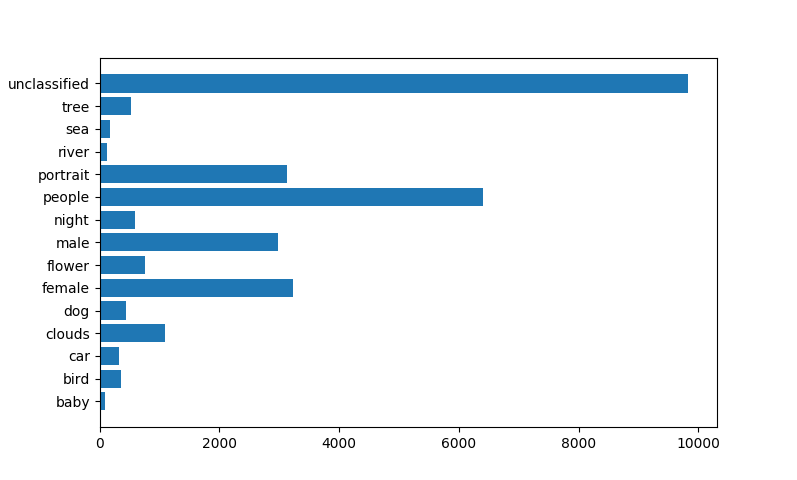
\includegraphics[height=0.6\textheight]{images/label_distribution.png}
		\caption{Class distribution}
		\end{figure}
	\end{itemize}
\end{frame}

\begin{frame}
	\frametitle{Methods}
	\framesubtitle{Class weights 2/2}
	\begin{itemize}
			\item We tackled this problem by custom weights per class
			\begin{itemize}
				\item Giving them at training phase
			\end{itemize}
		\end{itemize}
	\begin{block}{Class weight function}
	\begin{align*}
	S(c_i;\lambda) = \ln\left(\lambda \dfrac{\sum_{c}|c|}{|c_i|}\right)\\\\
	W(c_i; \lambda) = \max(S(c_i;\lambda), 1)
	\end{align*}
	\end{block}
\end{frame}

\begin{frame}
	\frametitle{Methods}
	\framesubtitle{Network topology}
	\begin{itemize}
		\item One network that outputs 15 classes
		\item Three convolution layers all followed by max pooling
		\begin{itemize}
			\item Filters 32, 32, 64
			\item Kernel size $3 x 3$
			\item Max pool size $2 x 2$
			\item ReLu as activation function
		\end{itemize}
		\item After pooling flattening via dropout to dense layer with sigmoid activation
		\begin{itemize}
			\item Dropout value: 0.4
		\end{itemize}
		\item Very simple network
	\end{itemize}
\end{frame}

\begin{frame}
	\frametitle{Methods}
	\framesubtitle{Loss function 1/2}	
	\begin{itemize}
		\item Categorical crossentropy wouldn't work as one image can be in many classes
		\item Binary crossentropy was suggested in many forum posts				
			\begin{itemize}
				\item Still not viable solution when there are many overlapping categories
				\item Loss is too forgiving for giving 0 labels
			\end{itemize}
	\end{itemize}
\end{frame}

\begin{frame}
	\frametitle{Methods}
	\framesubtitle{Loss function 2/2}
	\begin{itemize}
				\item Solution: "custom" loss function \textbf{BP-MLL}\footnote{Backpropagation for Multilabel Learning}
		\begin{itemize}
			\item Actually taken directly from the paper [1]\footnote{[1] \emph{Multilabel Neural Networks with Applications to Functional Genomics and Text Categorization}, 2006}
			\item Designed for multi-label problems
			\item Implementation for Keras can be found from internet
			\item Punishes more from just giving 0 labels
		\end{itemize}
	\end{itemize}
	\begin{block}{}
			$$ E =  \sum_{i=1}^{m} \dfrac{1}{|Y_i||\bar{Y_i}|} \sum_{(k,l) \in Y_i \times \bar{Y_i}} \exp(-(c_k^i -c_l^i))$$
	\end{block}	
\end{frame}

\begin{frame}
	\frametitle{Methods}
	\framesubtitle{Validation}
	\begin{itemize}
		\item Per batch, 10\% of the data is randomly selected
		\item This subset is left out from the training phase
		\item Validated against in the final step
		\item With F1-score, we also inspected
		\begin{itemize}
			\item Binary accuracy
			\item Categorical accuracy
			\item Hamming loss
			\item Micro averaged precision score
		\end{itemize}
	\end{itemize}
\end{frame}